\documentclass{../../../lessonplan}
\renewcommand{\cflroot}{../../..}

\begin{document}

\lessonplantitle
    {KS1-S8}
    {Key Stage 1 Session 8}
    {Follow-own and extension work on multiple repeat loops and nested repeats}

\preamble
    {
    \item Understand and use simple repetition
    \item Use the repeat instruction several times in a program
    \item Use a repeat within a repeat loop (extension)
    }
    {
    \item Levels 23 to 25 in Rapid Router  
    \item Resource sheets KS1-S7-3, KS1-S8-1, and KS1-S8-2
    }
    {
    \item Repeat, repetition
    }

\begin{lessonplan}

The \keyword{repeat} loop is a key concept in computer programming.

This session consolidates understanding of the `repeat' loop, giving children a chance to work through levels 23 to 25.
Several of these levels require more than one \keyword{repeat} loop.
It also gives a chance for the more advanced children to look at the more complex `\keyword{repeat} within a \keyword{repeat}'.

Recap on level 22 \textit{[fig S8.1]} with the class.

\fig{fig S8.1}{figS8.1.jpg}{1}

\keyquestion{Can you sport parts of the route where blocks of code are repeated?}

This route includes up to six \keyword{repeat} loops for the forward instructions.

\subsection*{Main activity}

Give out resource sheet KS1-S7-3 \textit{[fig S8.2]} to those who have not tackled level 22 independently, and ask children in pairs to mark out the sections of the road where \keyword{repeat} could be used, recording their code.

\fig{fig S8.2}{figS8.2.jpg}{1}

Others will be able to tackle levels 23 and 24 using several \keyword{repeat} loops.

For gifted and talented pupils, look at level 23, where they can `nest' a \keyword{repeat} loop within a \keyword{repeat} loop.

Ask them to look at resource sheet KS1-S8-1 \textit{[fig S8.3]} and work out their algorithm using \keyword{repeat}.

\fig{fig S8.3}{figS8.3.jpg}{1}

They will probably come up with:

\begin{center}
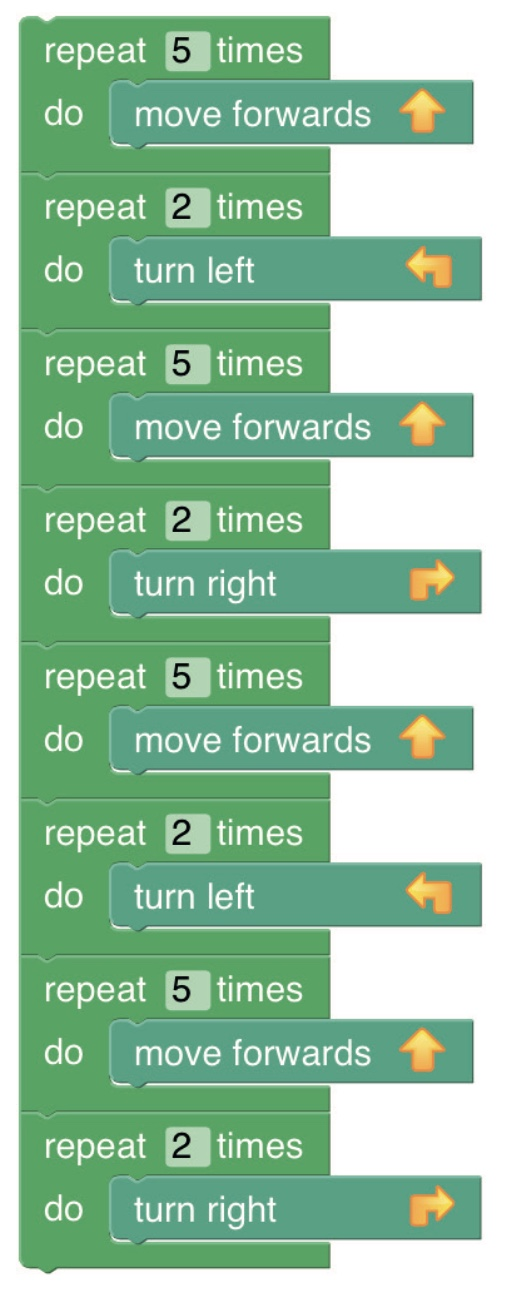
\includegraphics[width=.667\linewidth]{example1.jpg}
\end{center}

Can they see another \keyword{repeat} pattern here?
They may see that it is repeated twice, so you could put that sequence inside a repeat loop.

\begin{center}
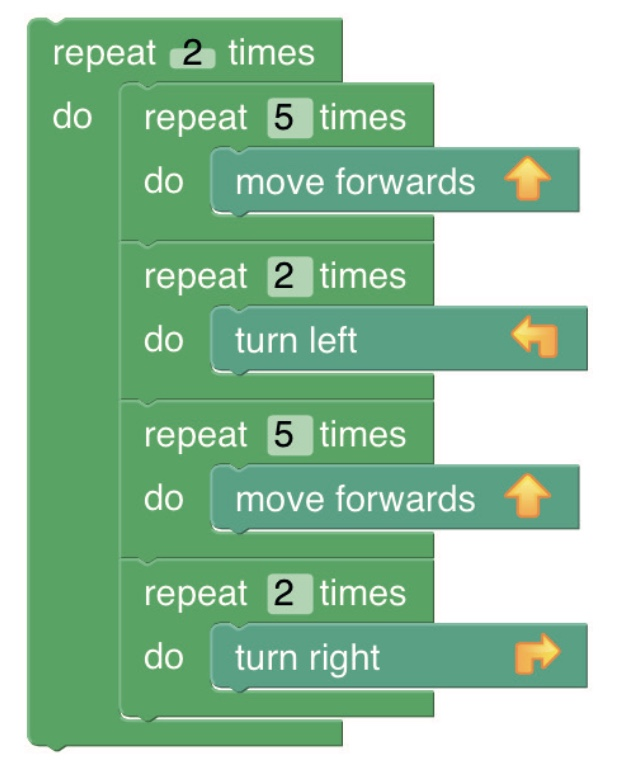
\includegraphics[width=.667\linewidth]{example2.jpg}
\end{center}

\section*{Unplugged activity for gifted and talented pupils}

Give gifted and talented children resource sheet KS1-S8-2 \textit{[fig S8.4]} on nested repeat with this code, and ask them to draw the route.

\fig{fig S8.4}{figS8.4.jpg}{1}

\begin{center}
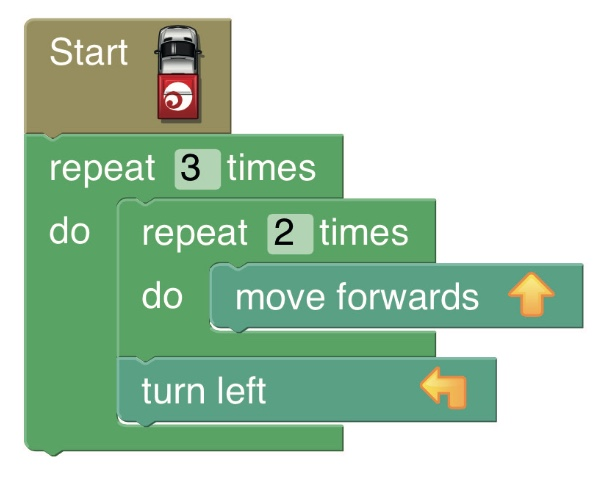
\includegraphics[width=.667\linewidth]{example3.jpg}
\end{center}

This is the solution \textit{[fig S8.5]}.

\fig{fig S8.5}{figS8.5.jpg}{1}

\end{lessonplan}

\end{document}
